\newtheorem{theorem}{Theorem}
\newtheorem{problem}{Problem}
\renewcommand\proofname{Proof}

\section{Problem definition}

First, the problem will be formalized and will be referred to as Detecting-Inversions. 

\begin{problem}[Detecting-Inversions]
\noindent \\
{\bf INPUT:} a collection of sample-specific strings for a target sequence $T$ and a reference $R$. \\
{\bf OUTPUT:} a list of disjoint segments $T[i,j]$ that are inverted in relation to the reference sequence $R$. 
\end{problem}

The main idea of the algorithm is that the target is a long read coming from a genome $G$ that differs from the reference $R$ by possible operations of inversions. Such operations will be non-overlapping, meaning repeated inversions in overlapping positions will not be considered. \\ 

\section{Pseudocode}

\begin{algorithm}[H]
\caption{Check For Inversions Using Sample-Specific Strings}
\hspace*{\algorithmicindent} \textbf{Input: } target: string, reference: string, indexes: list of integers, lengths: list of integers, sample\_specific\_strings: list of strings \\
\hspace*{\algorithmicindent} \textbf{Output: } reverted: list of reverted sequences found 
\begin{algorithmic}[1]
\STATE reverted $\gets$ [ ] \COMMENT{Initialize list to store inversions}
\FOR{$i \gets 1$ \TO $\text{sample\_specific\_strings.length} - 1$}
    \STATE $j \gets \text{indexes}[i]$ \COMMENT{Start index of current sample-specific string (SFS)}
    \STATE $k \gets \text{indexes}[i + 1]$ \COMMENT{Start index of next SFS}
    \STATE middle $\gets$ target$[j + \text{lengths}[i]:k]$ \COMMENT{Extract potential inversion}
    \IF{middle $==$ $\emptyset$}
        \STATE \textbf{CONTINUE}
    \ENDIF
    \STATE middle $\gets$ \textbf{REVERT\_AND\_COMPLEMENT}(middle)
    \STATE (found, start) $\gets$ \textbf{CHECK\_SUBSTRING}(reference, middle) \COMMENT{Search in reference}
    
    \IF{found}
        \STATE left\_increment $\gets 1$
        \WHILE{$\text{left\_increment} \leq \text{lengths}[i]$ \AND $(j + \text{lengths}[i] - \text{left\_increment}) \geq 0$ \AND target$[j + \text{lengths}[i] - \text{left\_increment}] == \textbf{REVERT\_AND\_COMPLEMENT}(\text{reference}[\text{start} + \text{middle.length} + \text{left\_increment} - 1])$}
            \STATE left\_increment $\gets$ left\_increment $+ 1$ \COMMENT{Extend left breakpoint}
        \ENDWHILE
        \STATE left\_breakpoint $\gets$ target$[j + \text{lengths}[i] - \text{left\_increment}: j + \text{lengths}[i] - \text{left\_increment} + 2]$
        
        \STATE right\_increment $\gets 0$
        \WHILE{$\text{right\_increment} < (\text{reference.length} - \text{start} - \text{middle.length})$ \AND $(k + \text{right\_increment}) < \text{target.length}$ \AND target$[k + \text{right\_increment}] == \textbf{REVERT\_AND\_COMPLEMENT}(\text{reference}[\text{start} - 1 - \text{right\_increment}])$}
            \STATE right\_increment $\gets$ right\_increment $+ 1$ \COMMENT{Extend right breakpoint}
        \ENDWHILE
        \STATE right\_breakpoint $\gets$ target$[k + \text{right\_increment} - 1: k + \text{right\_increment} + 1]$
        
        \STATE inversion $\gets$ target$[j + \text{lengths}[i] - \text{left\_increment} + 1: k + \text{right\_increment}]$
         \vspace{-2.9ex} 
        \STATE \textbf{APPEND} reverted $\gets$ inversion \COMMENT{Store the inversion}
    \ENDIF
\ENDFOR
\RETURN reverted
\end{algorithmic}
\end{algorithm}





\begin{algorithm}[H]
\caption{Revert and Complement DNA Sequence}
\hspace*{\algorithmicindent} \textbf{Input: } DNA sequence: string \\
\hspace*{\algorithmicindent} \textbf{Output: } reverse and complement sequence: string
\begin{algorithmic}[1]


\STATE $\text{complements} \gets \{ 'A': 'T', 'C': 'G', 'G': 'C', 'T': 'A' \}$
\STATE $\text{reverted\_complement} \gets \varepsilon$

\FOR{$i \gets \text{sequence.length} - 1$ \TO $0$}
    \STATE $base \gets \text{sequence}[i]$
    \STATE $complement \gets \text{complements}[base]$
    \STATE $\textbf{APPEND} \text{ reverted\_complement} \gets complement$
\ENDFOR

\RETURN $\text{reverted\_complement}$
\end{algorithmic}
\end{algorithm}


\begin{algorithm}[H]
\caption{Knuth-Morris-Pratt Prefix Function}
\hspace*{\algorithmicindent} \textbf{Input: } pattern: string \\
\hspace*{\algorithmicindent} \textbf{Output: } LPS array: list of integers

\begin{algorithmic}[1]
\STATE $m \gets \text{length of pattern}$
\STATE $lps \gets [0] * m$ 
\STATE $j \gets 0$ 
\STATE $i \gets 1$
\WHILE{$i < m$}
    \IF{$\text{pattern}[i] == \text{pattern}[j]$}
        \STATE $j \gets j + 1$
        \STATE $lps[i] \gets j$
        \STATE $i \gets i + 1$
    \ELSE
        \IF{$j \neq 0$}
            \STATE $j \gets lps[j - 1]$
        \ELSE
            \STATE $lps[i] \gets 0$
            \STATE $i \gets i + 1$
        \ENDIF
    \ENDIF
\ENDWHILE
\RETURN $lps$
\end{algorithmic}
\end{algorithm}

\begin{algorithm}[H]
\caption{Check Substring Using Knuth-Morris-Pratt}
\hspace*{\algorithmicindent} \textbf{Input:} reference: string, string: string \\
\hspace*{\algorithmicindent} \textbf{Output:} Tuple of boolean (True if string is a substring of reference) and integer (starting index if found, -1 otherwise)

\begin{algorithmic}[1]
\STATE $n \gets \text{length of reference}$
\STATE $m \gets \text{length of string}$
\STATE $lps \gets \text{KMP Prefix Function}(string)$

\STATE $i \gets 0$ 
\STATE $j \gets 0$ 

\WHILE{$i < n$}
    \IF{$\text{string}[j] == \text{reference}[i]$}
        \STATE $i \gets i + 1$
        \STATE $j \gets j + 1$
    \ENDIF

    \IF{$j == m$}
        \RETURN $(\text{True}, i - j)$ 
    \ELSIF{$i < n$ \AND $\text{string}[j] \neq \text{reference}[i]$}
        \IF{$j \neq 0$}
            \STATE $j \gets lps[j - 1]$
        \ELSE
            \STATE $i \gets i + 1$
        \ENDIF
    \ENDIF
\ENDWHILE
\RETURN $(\text{False}, -1)$ 
\end{algorithmic}
\end{algorithm}

\newpage
\section{High-Level Explanation}

The algorithm for solving the Detecting-Inversions problem is structured in a way that involves different phases, as d
etailed below. The approach assumes solving the Detecting-Inversions problem starting from SFSs. \\
The algorithm addresses an auxiliary problem where the input data has the additional information given by a list of SFSs of the target with respect to the reference $R$.\\
It is important to note that each SFS represents a substring that does not occur in $R$, and potentially each SFS is used to capture the breakpoints of an inversion. The algorithm proceeds as follows:

\begin{itemize}
    \item \textbf{Setup (line 1):} 
     an empty list, \( reverted \), is initialized to store any detected inverted sequences. This list ensures that only valid inverted segments are stored throughout the process.
    \item \textbf{Iterate through SFS pairs and extraction of the segment (lines 2-8):} the algorithm focuses on the prime candidate for detecting inversions, which is the segment between a couple of sample-specific strings. Therefore, the core of the algorithm involves iterating through each pair of adjacent sample-specific strings. It confronts every pair \( (x, y) \) of sample-specific strings within the range, where \( x = S[i_j : i_j + l_j] \) and \( y = S[i_{j+1} : i_{j+1} + l_{j+1}] \), and extracts the segment \( m \) that lies exactly in the middle of the two sample-specific strings \( x \) and \( y \). More precisely, \( m = S[i_j + l_j : i_{j+1}] \). The extracted segment \( m \) represents the region that could potentially be the inversion.
    \item \textbf{Reverse Complement Generation (line 9):} when handling genomic data, an inversion is not just a reversal of the nucleotide sequence, but it also involves the complementing of bases, as seen on Chapter 2. After extracting the middle segment \( m \), its reverse complement \( m_r \) can be easily obtained: first, the bases in \( m \) are reversed, then each base is replaced with its complement (see Algorithm 3). The segment \( m_r \) is the transformed version of \( m \) that allows the algorithm to search for inverted regions in \( R \). 
    \item \textbf{Search for the reverse complement in the reference string (line 10): } the logic behind this step is that if \( m \) is actually an inverted segment, this means that its reverse and complement \( m_r \) can be found within the reference \( R \), since \( R \) represents the original, non-inverted version of the sequence. To efficiently locate \( m_r \) in \( R \), the algorithm uses the KMP algorithm, detailed in Chapter 2. If \( m_r \) is found in \( R \), the starting index \( s \) of the occurrence of \( m_r \) in \( R \) is stored for further analysis. 
    \item \textbf{Identify breakpoints (lines 12-23): } the identifications of breakpoints is essential to precisely locate the boundaries of the inversion within the target sequence \( S \). So, if the reverse complement \( m_r \) is found in \( R \), the algorithm proceeds to identify the inversion breakpoints, that define the boundaries of the inverted segment in \( S \). The breakpoints are determined by comparing characters from \( S \) and \( R \) in two stages:
    \begin{itemize}
    	\item \textbf{Left Breakpoint Identification (lines 12-16):} starting from the last character of the first sample-specific string \( x \) in \( S \), that corresponds to \( S[i_j + l_j] \) and the first character immediately following \( m_r \) in \( R \), which is \( R[s + m_r .length] \), the algorithm compares corresponding characters from \( S \) and the reverse complement of \( R \). This comparison continues backward in \( S \) and forward in \( R \) until a mismatch occurs. At this point, the final position in \( S \) is marked as left breakpoint.
    	\item \textbf{Right Breakpoint Identification (lines 17-21):} the right breakpoint is determined symmetrically. The comparison starts from the first character of the second sample-specific string \( y \) in \( S \), \( S[i_{j+1}] \), and the character immediately preceding \( m_r \) in \( R \), \( R[s - 1] \), and the search proceeds forward in \( S \) and backward in \( R \) until a mismatch is found, marking the right breakpoint in \( S \). 
    \end{itemize}
\end{itemize}




\section{Preconditions for Algorithm Correctness}

For this algorithm to function correctly, the middle segment extracted from the target must be sufficiently long to ensure its uniqueness within the reference sequence. This is crucial, because a middle segment that is too short might match multiple locations within the reference sequence, leading to a potential misalignment. This means that the algorithm might identify incorrect breakpoints or even wrongly identify an inversion that does not actually exist, resulting in a false positive. \\
A second prerequisite for algorithm accuracy is that the target sequence, and particularly the middle segment, must be free of errors or mutations. In fact, even a single error within the middle segment can disrupt the transformation process where the segment is reversed and complemented. As a result, the transformed segment might not match the expected part of the reference sequence, leading to false negatives where actual inversions are missed. 

\section{Edge Cases}
An important edge case to consider occurs when two sample-specific strings appear consecutively without any intervening characters in the target string. In this scenario, the middle segment will be an empty string. This happens because there are no characters between the end of the first sample-specific string and the beginning of the second one. An example is given below:

\begin{example}
  This is an example of the edge case where the two sample-specific strings are consecutive:
\begin{itemize}
    \item \textbf{Sample-specific strings: } 'S1', 'S2'
    \item \textbf{Target string: }  '\dots S1S2\dots'
\end{itemize}
\end{example}


In this case the starting index of 'S1' is \textit{j} and the starting index of 'S2' is \textit{k}, making the middle segment target[\textit{j} + S1.length : \textit{k}], which evaluates to an empty string.

\section{Proof of Correctness}

Now that the algorithm has been explained in detail, the proof of its correctness will be provided. \\
Let \( S = xyz \) be a string, where \( x \), \( y \), and \( z \) are substrings of \( S \): Let also \(y^r \) be the reversal of \( y \). The aim is to demonstrate that it is possible to reconstruct the sequence \( S' = z^r y^r x^r \), where the superscript '\( r \)' indicates the reversal of a string. For the sake of simplicity, the complement will be ignored. The proof will be made using mathematical induction. 

\begin{figure}[h]

  \centering
    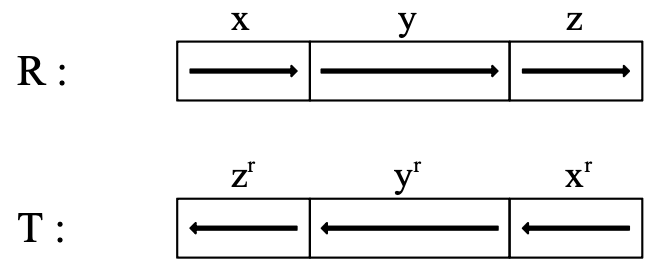
\includegraphics[width=300px]{rev.png}

  \caption{\( R \) represents the reference string, that in the following demonstration will be referred as \( S \), and \( T \) is the target where the inversion is found, that will be later referred as \( S' \).}
  \label{fig:rev}

\end{figure}

\begin{theorem}
    For any string \( S = xyz \), where \( x \), \( y \), \( z \) are substrings of \( S \), given \(y^r \), reversal of \(y\), it is possible to reconstruct the sequence \( S' = z^r y^r x^r \). 
\end{theorem}
\paragraph{Proof}
\\ 
\textbf{Base case: } \|\( y \)\| = 1 \\
\\ Let \( \| y \| = 1 \), meaning \( y \) only consists of a single character '\( a \)'. In this trivial case, \( S = xaz \), and \(y^r \) = \( a \). Hence, the string \( S' = z^r y^r x^r \) can be reconstructed as follows: 
\begin{enumerate}
\item Reverse \( z \) to obtain \( z^r \);
\item Append \( y^r \), which is simply '\( a \)';
\item Append the reversal of \( x \), which is \( x^r \).
\end{enumerate}
The resulting sequence \( S' \) is \(z^r a x^r \), equivalent to \( S' = z^r y^r x^r \) when \|\( y \)\| = 1. \\
\\ \textbf{Inductive step: } \( \| y \| > 1 \) \\

\\ Assume that for some \( k > 1 \), it is possible to reconstruct \( S' = z^r y^r x^r \) when \( \| y \| = k \) (inductive hypothesis). It will be proven that this reconstruction is also possible when \( \| y \| = k + 1 \). 

Let \( y = a_1 a_2 \dots a_k a_{k+1} \), where each \( a_i \) is a single character. Thus, \( y^r = a_{k+1} a_k \dots a_2 a_1 \). According to the inductive hypothesis, it is possible to reconstruct \( S' = z^r (a_1 a_2 \dots a_k)^r x^r \). In order to obtain \( S' = z^r y^r x^r \) for \( \| y \| = k + 1 \), the following steps are necessary:
\begin{enumerate}
    \item Start with \( z^r (a_k \dots a_2 a_1) x^r \);
    \item Insert \( a_{k+1} \) before \( a_k \dots a_2 a_1 \);
\end{enumerate}
The result is \( z^r (a_1 a_2 \dots a_k a_{k+1})^r x^r \), which corresponds to \( S' = z^r y^r x^r \) for \( \| y \| = k + 1 \).


\section{Time and Space Complexity}
This analysis will start with time complexity. \\
During the initialization phase, the necessary parameters are set up, and the list for storing the reverted sequences is initialized. These steps are performed in constant time, hence $\mathcal{O}(1)$. \\

In the iteration phase, each pair of sample-specific strings is processed. Let \( n \) denote the total number of sample-specific strings, each interaction involves the extraction of the segment \( m \) between two adjacent sample-specifics strings. This step is repeated for each pair, and extracting the segment takes a time that is proportional to its average length $\bar{m}$, so the overall time complexity of this phase is $\mathcal{O}(n \cdot \bar{m} )$. \\

In the following phase, the middle segment is transformed by reverting its characters and complementing each base. This operation takes $\mathcal{O}( \bar{m})$ time per iteration, so the overall time complexity of this phase is, just like the previous one, $\mathcal{O}(n \cdot \bar{m} )$. \\

For the search in the reference string, the KMP algorithm is used to locate the transformed segment \( m_r \) within the reference \( R \). First, the LPS array is constructed. The array is initialized of size \( m \), where \( m \) is the length of the pattern. Keeping in mind that this data may vary when multiple inversions having different lengths are found during the whole computation, the actual value analyzed here is the average length \( \bar{m} \).  Then, the algorithm iterates through the pattern and the LPS array is filled based on the comparison of the characters in the pattern. Each character is processed at most twice: once when a match is found, and again if a mismatch occurs (when the pointer \( j \) is reset based on the LPS array). Therefore, the time complexity required for the LPS computation is $\mathcal{O}(\bar{m})$, hence linear. \\
Once the LPS array has been built, the actual search of the substring begins, iterating over the characters in the reference string, while using the information in the LPS array in order to skip unnecessary comparisons. Each character in the reference string is processed at most once. Additionally, the character comparisons are skipped according to the values in the LPS array. Therefore, said \( r \) the length of the reference, the time complexity of the search is  $r + \mathcal{O}(\bar{m})$, which also makes the total time complexity of the whole phase. \\

In the last phase, the algorithm identifies the left and right breakpoints, which requires comparing characters in both target and reference sequences. Considering the search of the left breakpoint, where the algorithm starts at the last character of the first sample-specific string in the target and the character immediately following the segment in the middle segment extracted in the reference, the number of comparisons performed depends on the length of the first sample-specific string. Said \( s \) such length, in the worst case scenario, the algorithm compares \( s \) characters. The process is the same for the right breakpoint, but the length of the second sample-specific string may differ. Therefore, the time complexity must be proportional to the average length of the sample-specific strings, that will be referred as $\bar{s}$. Since the algorithm iterates over \( n \) sample-specific strings, the total time complexity of this phase is $\mathcal{O}(n \cdot \bar{s} )$. \\

The overall time complexity is determined combining all the phases. Therefore, it can be expressed as $\mathcal{O}(n \cdot \bar{m} + n \cdot \bar{m} + r + \bar{m} + n \cdot \bar{s})$ and summarized as $\mathcal{O}(n \cdot \bar{m} + r + \bar{m} + n \cdot \bar{s})$. In this scenario, $\bar{m}$ is considerably smaller than the reference length  \( r \), and the same can be said of the average length of the sample specific strings \( \bar{s} \). Since the dominant terms that actually determine the total time complexity of the algorithm are $n \cdot \bar{m}$ and \( s \). Consequently, the result is $\mathcal{O}(r + n \cdot \bar{m} )$. \\


Regarding space complexity, the algorithm requires $\mathcal{O}(n \cdot \bar{m} )$ space to store the list of reverted sequences. Additionally, the LPS array used in the KMP algorithm demands $\mathcal{O}(\bar{m} )$ space for each segment processed and temporarily stored during the search phase. Temporary variables for indexing and counters occupy $\mathcal{O}(1)$ space. Although the middle segments are not stored long-term, the memory requirements are still significant due to the storage of reverted sequences. Therefore, the overall space complexity of the algorithm is $\mathcal{O}(n \cdot \bar{m} )$.
